\documentclass[letterpaper]{article}

\usepackage{natbib,alifeconf}  %% The order is important
\usepackage{url,hyperref,cleveref}
\usepackage{booktabs}

\newcommand\blfootnote[1]{%
  \begingroup
  \renewcommand\thefootnote{}\footnote{#1}%
  \addtocounter{footnote}{-1}%
  \endgroup
}

\title{A Million Combinator Reductions a Second: Hardware-Accelerated
Evolution of SKI Programs on Cloud FPGAs}

\author{
    Mark Santolucito$^{1}$,
    Christian Scaff$^{1}$,
    Andrew Bonilla$^{1}$, \and
    Zenas Boamah$^{1}$ \\
    \mbox{}\\
    $^1$Barnard PL Labs, Barnard College, Columbia University, USA \\
    msantolu@barnard.edu
}

\begin{document}

\maketitle

\begin{abstract}
    Evolutionary search over \emph{computation} --- programs, circuits,
    reaction networks --- is a recurring theme in artificial life, but it is
    chronically bottlenecked by the cost of \emph{evaluating} candidates. We
    present a massively-parallel evolutionary substrate that evolves SKI
    combinatory-logic programs entirely in FPGA fabric: each soft core
    generates, reduces (to weak head normal form via in-place graph reduction
    in block RAM), and scores candidates against a target function with no host
    in the inner loop. On a single low-cost ECP5 FPGA we measure
    \textbf{$>$1.0 million candidate evaluations per second} across 16 parallel
    cores, scaling linearly with core count, and synthesis shows ${\sim}60$
    cores fit on the device (a projected ${\sim}3.8$\,M\,eval/s). Against a
    bit-identical C implementation on a modern CPU (Apple M4), the FPGA matches
    a full chip's throughput at roughly \textbf{one-twelfth the power}, and the
    architecture projects to ${\sim}45$ datacenter-FPGA cards matching a
    100k-CPU farm at ${\sim}80\times$ lower power. The system is built and run
    entirely through \textbf{Manhattan Reasoning Gym (MRG)}, a cloud FPGA
    platform that lets researchers submit HDL and drive hardware over a simple
    SDK without owning boards --- lowering the barrier to hardware-accelerated
    artificial-life experiments. All designs and benchmarks are open.
\end{abstract}

% Choose one of: Full Paper, Summaries, or Late Breaking Abstracts
Submission type: \textbf{Late Breaking Abstracts}\\

Data/Code available at: \url{https://manhattanreasoning.com}
\blfootnote{\textcopyright  2026 The Authors. Published under a Creative Commons Attribution 4.0 International (CC BY 4.0) license.}

\begin{figure}[t]
    \centering
    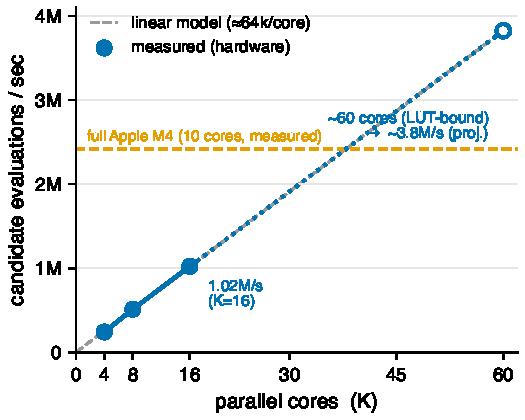
\includegraphics[width=0.72\columnwidth]{figures/fig1_scaling.pdf}
    \caption{Throughput scales linearly with on-chip cores. Three measured
    points ($K=4,8,16$) lie on a ${\sim}63.7$k-eval/s/core line; synthesis
    bounds the device at ${\sim}60$ cores (LUT-limited), projecting
    \textbf{${\sim}3.8$\,M\,eval/s} on one ${\sim}\$40$, ${\sim}3$\,W ECP5-85.
    The all-core Apple M4 is shown for reference; the FPGA passes a full modern
    CPU near 38 cores.}
    \label{fig:scaling}
\end{figure}

\section{Motivation}
Artificial life has a long tradition of \emph{evolving computation}: Tierra's
self-replicating machine code \citep{ray1991tierra}, Fontana \& Buss's AlChemy
(an algorithmic chemistry over $\lambda$-terms) \citep{fontana1994arrival}, and
the broader thread of algorithmic chemistries in which programs are the
molecules and reduction is the reaction. SKI combinatory logic is an especially
clean substrate for this lineage --- three primitives
(\texttt{S}, \texttt{K}, \texttt{I}), one operation (application),
Turing-complete, and free of variable binding, so terms are pure trees that
mutate and recombine trivially.

The persistent obstacle is \textbf{evaluation throughput}: evolutionary and
open-ended searches are dominated by the cost of reducing candidates and
scoring them, and richer experiments are simply unaffordable on CPUs at the
scales ALIFE questions often demand. We ask: \emph{what becomes possible if
candidate evaluation is $10^6$--$10^8$/sec?} Our answer is to move the entire
evolutionary inner loop --- generation, reduction, fitness --- onto FPGA
fabric, replicate it, and expose it through a cloud platform usable without
hardware.

\section{System}
\textbf{Substrate.} A candidate is a pure SKI term, stored as a graph of 32-bit
nodes in block RAM (tag $+$ two child pointers). The three rewrite rules are
$\texttt{I}\,x \to x$, $\texttt{K}\,x\,y \to x$, and
$\texttt{S}\,x\,y\,z \to x\,z\,(y\,z)$.

\textbf{On-chip evolutionary core.} Each soft core runs autonomously:
(1)~\emph{Generation} --- an LFSR drives a generator that writes a random
\emph{well-formed} term: every application node references only earlier nodes,
so terms are acyclic and in-range by construction. (2)~\emph{Reduction} --- a
weak-head-normal-form graph reducer unwinds the left spine with a 3-deep
sliding window (SKI's widest rule needs only three arguments, so no unbounded
stack), rewrites the head redex in place to preserve sharing, and guards
against non-termination with a per-candidate step cap. (3)~\emph{Fitness} ---
boolean targets use Church encodings ($\texttt{TRUE}=\texttt{K}$,
$\texttt{FALSE}=\texttt{K\,I}$), and the output is read by applying the
candidate to inert sentinel atoms. Fitness is the number of truth-table rows
matched; divergent or malformed candidates score zero by construction.

\textbf{Parallel engine.} $K$ cores share one Wishbone control interface; the
host writes the target and a seed, then reads a global candidate counter and
the best fitness found. There is \textbf{no host traffic in the inner loop} ---
the cores share nothing, so throughput tracks core count.

\textbf{Platform.} The whole thing is developed, built (Amaranth $\to$ Yosys
$\to$ nextpnr-ECP5 $\to$ bitstream), flashed, and driven through \textbf{Manhattan
Reasoning Gym}: HDL is submitted over an SDK, programmed onto an idle cloud
FPGA, and controlled with simple register reads/writes. No board ownership, no
local toolchain.

\section{Results}
All measurements: evolving 2-input XOR (\texttt{cand\_size}$=16$, step cap
2000), ${\sim}5$\,s free-running windows, on an ECP5-85
(\texttt{LFE5UM5G-85F}, 50\,MHz, ${\approx}\$40$, ${\approx}3$\,W).

\begin{table}[ht]
    \centering
    \begin{tabular}{rrrl}
        \toprule
        $K$ cores & cand./sec & per core & XOR \\
        \midrule
        4  & 241{,}670       & 60{,}417 & solved 4/4 \\
        8  & 512{,}152       & 64{,}019 & solved 4/4 \\
        16 & \textbf{1{,}021{,}698} & 63{,}856 & solved 4/4 \\
        \bottomrule
    \end{tabular}
    \caption{Throughput scales linearly with cores; the search solves the
    target at every $K$. Going $4\to16$ cores yields $4.23\times$ throughput at
    a flat ${\sim}63$k/s per core --- the cores are genuinely independent.}
    \label{tab:throughput}
\end{table}

\textbf{Resource scaling} (yosys \texttt{synth\_ecp5}). ${\sim}1{,}250$
LUT-equiv, 1 BRAM, 2 DSP per core, linear in $K$; LUTs bind first, so
\textbf{${\sim}60$ cores fit} on the ECP5-85. ($K=16$ is verified to route on
real silicon; place-and-route (${\sim}15$\,min) is the practical cost at high
$K$, not fabric.)

\textbf{Versus CPUs (bit-identical workload).} A C port (same generation,
reducer, and evaluation) on an Apple M4 measures ${\sim}320$k\,eval/s per core,
${\sim}2.42$\,M/s across the full chip (${\sim}22$\,W). Per \emph{core} the CPU
wins ${\sim}5\times$ --- purely clock (${\approx}88\times$ the 50\,MHz SoC) ---
but the FPGA core is \textbf{${\sim}18\times$ more cycle-efficient}
(${\sim}780$ vs ${\sim}14{,}000$ cycles/candidate): the datapath \emph{is} the
reducer. Net: one ${\sim}3$\,W ECP5 matches a 3\,nm flagship's whole-chip
throughput at \textbf{${\sim}12\times$ better eval/sec/W} (\Cref{fig:eff}).
Projected to datacenter FPGAs, \textbf{${\sim}45$ cards match a 100k-CPU farm
at ${\sim}80\times$ lower power and ${\sim}40$--$80\times$ lower cost}.

\begin{figure}[ht]
    \centering
    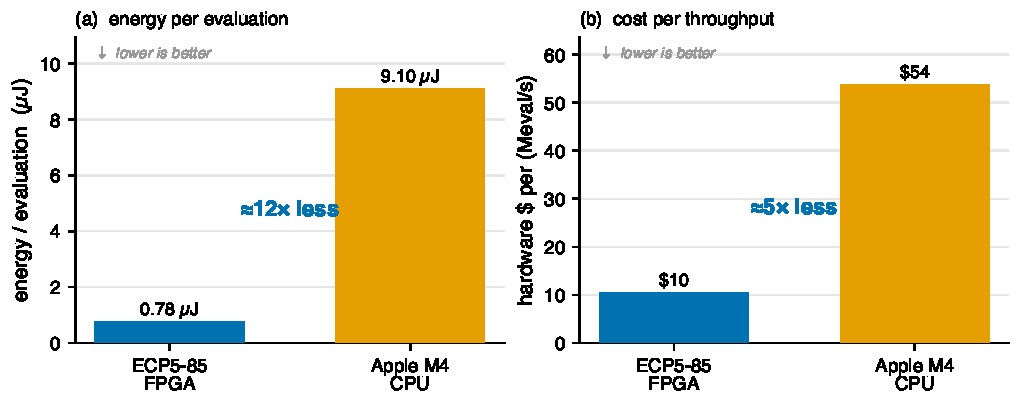
\includegraphics[width=0.88\columnwidth]{figures/fig2_efficiency.pdf}
    \caption{Total cost of ownership vs a modern CPU (bit-identical workload);
    both panels are clock-rate-independent cost-per-work, so lower is better.
    \textbf{(a)}~Energy per evaluation: ${\sim}12\times$ less
    (${\sim}0.78$ vs ${\sim}9.1\,\mu$J). \textbf{(b)}~Hardware \$ per sustained
    Meval/s: ${\sim}5\times$ less. Power (${\sim}3$/${\sim}22$\,W) and chip cost
    (${\sim}\$40$/${\sim}\$130$) are rough estimates; the gaps are robust to
    ${\sim}2\times$ uncertainty.}
    \label{fig:eff}
\end{figure}

\textbf{Why it works --- and where it doesn't.} The advantage is greatest when
candidates are \emph{small} (short terms, shallow truth tables, few
reductions). Hard monolithic targets (e.g.\ a 12-bit adder: $2^{24}$ rows) are
not a throughput problem but a \emph{search-strategy} one; the response is
decomposition --- evolve a small reusable cell, compose structurally.

\section{Future Work}
The reusable asset is the \textbf{engine architecture} --- generate $\to$
evaluate-on-fabric $\to$ select, massively parallel --- not the SKI substrate
specifically. Two directions.

\textbf{Combinator programs to circuits (evolvable hardware).} Swap the SKI
genome for the configuration vector of a \emph{virtual reconfigurable circuit}
--- a soft, runtime-programmable LUT/gate array (CGP-style
\citep{miller2011cgp}). A candidate loads in microseconds (no resynthesis) and
is evaluated as \emph{real} behavior on the fabric, so fitness can include
actual latency, switching activity, and active-cell count: the
intrinsic-evolvable-hardware tradition \citep{thompson1996evolved} at newly
affordable evaluation rates.

\textbf{ML-relevant primitives, with quality-diversity.} ML's tolerance for
approximation smooths the landscape and opens a large design space (approximate
MACs \citep{vasicek2015approximate}, stochastic-computing elements, systolic
tiles). MAP-Elites search \citep{mouret2015illuminating} would \emph{illuminate}
an accuracy-vs-area-vs-power map rather than return a single winner --- a
natural fit for open-ended ALIFE methods, and a path to evolving hardware that
accelerates ML \citep{fawzi2022alphatensor}. Large structures will need
developmental/generative encodings.

\section{Availability}
The SKI evaluator, parallel GA engine, CPU baseline, and benchmarks are open
and reproducible on \textbf{Manhattan Reasoning Gym} \citep{mrg2026}: submit a
design, program a cloud FPGA, and drive the search with a few register writes
--- inviting others to evolve in fabric.

\footnotesize
\bibliographystyle{apalike}
\bibliography{alife-lbw}

\end{document}
